\begin{abstract}
近年、実験技術の発展により冷却原子系における熱平衡化が実験で観測され、理論と実験の両方から量子系の非平衡過程への理解が進んでいる。量子系での非平衡過程を理論的に取り扱うことは、エンタングルメントと呼ばれる量子情報理論的な現象により相互作用が弱い場合でさえも容易ではなく、量子情報理論的なアプローチから非平衡過程を理解する理論研究が活発になされている。そこで我々は新たに、強結合でカオス性の強い1+1次元共形場理論を\textcircled{\scriptsize 1}分離クエンチをしたときの\textcircled{\scriptsize 2}エンタングルメントエントロピー(EE)の時間発展を計算した。
\begin{enumerate}
	\item クエンチとは、ある量子系のハミルトニアンの基底状態を用意して、瞬時にハミルトニアンを変化させることを指す。用意された基底状態はクエンチによって励起状態となり、クエンチ後のハミルトニアンの基底状態へと熱平衡化していく。$N$重分離クエンチとは、ある$N$点での相互作用を“切る”ことで、瞬時に量子系を$N+1$個に分離するクエンチのことである。
	\item エンタングルメントエントロピー(EE)とは注目系とそれ以外の系とのエンタングルメントの度合いを測る量であり、これを用いることでエンタングルメントに起因する量子系の非平衡過程を調べることができる。超弦理論から予想されたAdS/CFT対応を用いることで、AdS時空に双対となるような共形場理論(CFT)でのEEを、AdS時空内の測地線の長さを用いて計算することができる。AdS時空に双対となる共形場理論は、強結合でカオス性が強い量子系の臨界点での物理を記述する理論であると考えられており、冷却原子系への応用を考える上でも興味深い。
\end{enumerate}

我々の研究\cite{Shimaji:2018czt}\cite{Caputa:2019avh}では新たに、AdS時空に双対となる共形場理論の真空に対して接合/分離クエンチと2重接合/分離クエンチをしたときのEEの時間発展を、AdS空間内の測地線の長さを計算することで解析した。

本論文では分離クエンチ・2重分離クエンチに焦点を当てて、その解析結果を解説する。共形場理論に生じた分離によって、その双対なAdS時空にも分離が生じることが分かった。そしてこの描像を用いて、2重分離クエンチのEEを調べることでAdS$_3$時空の境界の重力相互作用の存在を予想した。
\end{abstract}

\tableofcontents

\chapter{導入}
\section*{ブラックホールエントロピーとAdS/CFT対応}
1973年にBekenstein\cite{Bekenstein:1973ur}によってブラックホールの面積の持つ性質と熱力学のエントロピーの性質の類似が指摘された。その後、Hawking,Unruh,Gibbons,Yorkらの研究\cite{Hawking:1974sw}\cite{Unruh1976}\cite{Bekenstein:1974ax}\cite{Gibbons:1976ue}\cite{York:1986it}によって、重力を半古典近似すればブラックホールはある温度(Hawking温度と呼ばれる)で黒体のように輻射しており、さらにブラックホールのエントロピーが
\begin{align}
S_{BH}=\frac{k_B c^3}{4G \hbar}\text{Area}(\text{horizon})
\end{align}
で表されることが分かった。このブラックホールエントロピーは\textbf{Bekenstein-Hawkingエントロピー}と呼ばれる。Bekenstein-Hawkingエントロピーは右辺にプランク定数を含むため、重力の量子論に対する指導原理の一つとして考えられている。また、Bekenstein-Hawkingエントロピーは表面積に比例するが、しかし通常の物質のエントロピーはその体積に比例する(示量性)ことが経験的に知られている。このことはブラックホールの内部の自由度があたかも表面のみで代表されることを示唆しており、Bekenstein-Hawkingエントロピーの式を統計力学的な導出から理解をすることを動機づけた。これによってBombelliら\cite{Bombelli:1986rw}やSrednicki\cite{Srednicki:1993im}によって場の量子論でのエンタングルメントエントロピーの解析が始まった。多くの研究によって場の理論のエンタングルメントエントロピーも面積に比例することが分かった。しかし場の理論のエンタングルメントエントロピーは紫外発散を含むので、ブラックホールエントロピーをブラックホール時空上の場の理論のエンタングルメントエントロピーとして解釈することはできない。しかし後に実はエンタングルメントエントロピーはブラックホールエントロピーの量子補正として解釈できることが分かった\cite{Solodukhin:2011gn}。また、この流れはHolzey, Larsen, Wilczek\cite{Holzhey_1994}による2次元共形場理論のエンタングルメントエントロピーの研究につながり、Calabrese, Cardy\cite{Calabrese:2004eu}\cite{Calabrese:2005in}によって物性理論へも応用されている。

1995年にPolchinski\cite{Polchinski:1995mt}によって超弦理論でのDブレーンが発見されると、Dブレーンを置いた超弦理論の低エネルギー極限としてブラックホールが記述できることが分かり、Strominger, Vafa\cite{Strominger:1996sh}によってAdS時空でのブラックホールのエントロピーが超弦理論での状態の数え上げから導出された。その後、Maldacena\cite{Maldacena:1997re}によってその枠組みは\textbf{AdS/CFT対応}へと昇華された。AdS/CFT対応は$d+1$次元の反de Sitter(AdS)時空上の量子重力理論」と「AdS時空の$d$次元の境界の上の共形場理論(CFT)」との等価性を主張し、$d+1$次元AdS時空のブラックホールは有限温度の$d$次元共形場理論に等価になる。したがってBekenstein-Hawkingエントロピーは有限温度の場の理論でのエントロピーとして解釈され、ブラックホール熱力学は単に場の理論での熱力学に対応することが分かった。しかし、この枠組みはあくまでAdS時空でのブラックホールに対する理論である。AdS時空でのブラックホールはde Sitter時空やMinkowski時空上のブラックホールとは異なり、Hawking放射によって蒸発しなかったり、宇宙定数が負であったりと、現実のブラックホールのモデルであるとは考えられていない。しかしAdS/CFT対応は、強結合で閉じ込めが起きるような共形場理論を古典AdS重力によって簡単に解析することを可能にし、QCD\cite{Sakai:2004cn}\cite{Kovtun:2004de}や強相関物性系\cite{Hartnoll_2009}への応用が考えられている。

2006年に笠,高柳によって発見されたホログラフィックなエンタングルメントエントロピーの\textbf{笠-高柳公式}\cite{Ryu:2006ef}は、AdS/CFT対応を用いて共形場理論でのエンタングルメントエントロピーをAdS空間の極小曲面の面積に関係づける公式で、
\begin{align}
S_\text{entanglement entropy}=\frac{k_B c^3}{4G \hbar}\text{Area}(\text{extremal surface})
\end{align}
と表される。AdS/CFT対応から、ブラックホールエントロピーは共形場理論の有限温度状態のエントロピーとして解釈できたが、この式はその一般化になっている。この公式はAdS/CFT対応を用いた量子重力理論への情報理論的なアプローチのみならず、強結合な場の理論でのエントロピーの解析にも応用されているなど、最近の理論研究の新たな潮流となってきた。

\section*{共形場理論における量子クエンチ}
量子系における熱平衡化の研究は、量子力学に基づく系の熱力学的な性質の理解につながるため、様々な物理の分野において長年にわたって研究されている。その中でも、外部系(熱浴)と相互作用していない孤立量子系において``熱平衡化"が起きるかという問題は1929年に既にvon Neumann\cite{Neumann1929}\cite{von_Neumann_2010}によって指摘されていたが、現在この問題は「量子多体系のエネルギー固有状態が熱平衡状態に近似できる」とする固有状態熱化仮説(eigenstate thermalization hypothesis, ETH)\cite{Deutsch1991}\cite{Srednicki1994}とともに再び注目を集めている。

孤立量子系の熱平衡化の重要性が見直された背景には、実験技術の進歩の貢献が大きい。1980年代に大きく発展したレーザー冷却\cite{Phillips1998}\cite{Metcalf2007}の実験技術によって、レーザーによってトラップされBose-Einstein凝縮した冷却原子系を実現することが可能になった。冷却原子系は孤立量子系を実験的に実現しており、その熱平衡化過程も実験的に調べられるようになったのである。

冷却原子系の実験では、様々な状態を用意したり、系のハミルトニアンの外部パラメータを簡単に変化させることができる。冷却原子系での熱平衡化を調べる典型的なセットアップの一つは、外部磁場などのパラメータを瞬時に変化させて系の状態を平衡状態からずらし(これを\textbf{クエンチ(quench)}と呼ぶ)、新たな平衡状態へ緩和する過程を調べるというものである。様々なクエンチを起こし方に対する物理量の変化を調べる研究は実験\cite{greiner2002collapse}\cite{kinoshita2006quantum}\cite{hofferberth2007non}\cite{trotzky2012probing}\cite{cheneau2012light}\cite{gring2012relaxation}、理論\cite{essler2016quench}\cite{Calabrese2006}\cite{fagotti2013}\cite{manmana2007}の双方から盛んに調べられている。

2次元共形場理論でのクエンチを考えることは、臨界点上の冷却原子系の振る舞いを調べられるだけでなく、AdS/CFT対応を用いてブラックホール時空に関連した熱平衡化過程を調べられるようになるという点で興味深い。とくにCalabrese, Cardyによって導入された、2次元共形場理論での大域クエンチ(global quench)\cite{Calabrese:2007rg}の問題設定は、高柳、宇賀神\cite{Takayanagi:2010wp}やHartman, Maldacena\cite{hartman2013time}らなどによってAdS/CFT対応を通してブラックホール生成過程の問題として解釈されたりしている。

\section*{我々の結果}
我々の研究\cite{Shimaji:2018czt}\cite{Caputa:2019avh}で注目したのは、2次元共形場理論での\textbf{局所クエンチ(local quench)}である。大域クエンチが系全体のハミルトニアンを瞬時に変化させることであるのに対し、局所クエンチとは系に瞬時に局所的な励起を与えることを指す。

1つ目の研究\cite{Shimaji:2018czt}では、我々は「接合」・「分離」の2つのタイプの局所クエンチによるエンタングルメントエントロピー(EE)の時間発展と、その重力双対である測地線の時間発展を考えた。

2つ目の研究\cite{Caputa:2019avh}では、我々は「接合」・「分離」の2つのタイプの2重局所クエンチによるエンタングルメントエントロピー(EE)の時間発展を解析し、2重接合クエンチについては重力双対の描像を考えた。

「接合」・「分離」の局所クエンチとは、時刻$t=0$である一点$x=x_1$において、「2つの半直線上の共形場理論の真空を接合する」・「直線上の共形場理論の真空を2つに分離する」クエンチのことを指し、また、2重クエンチとはそれらのクエンチが異なる2点$x=x_1,x_2$で同時に起きるモデルを指す。
\begin{figure}[H]
	\centering
	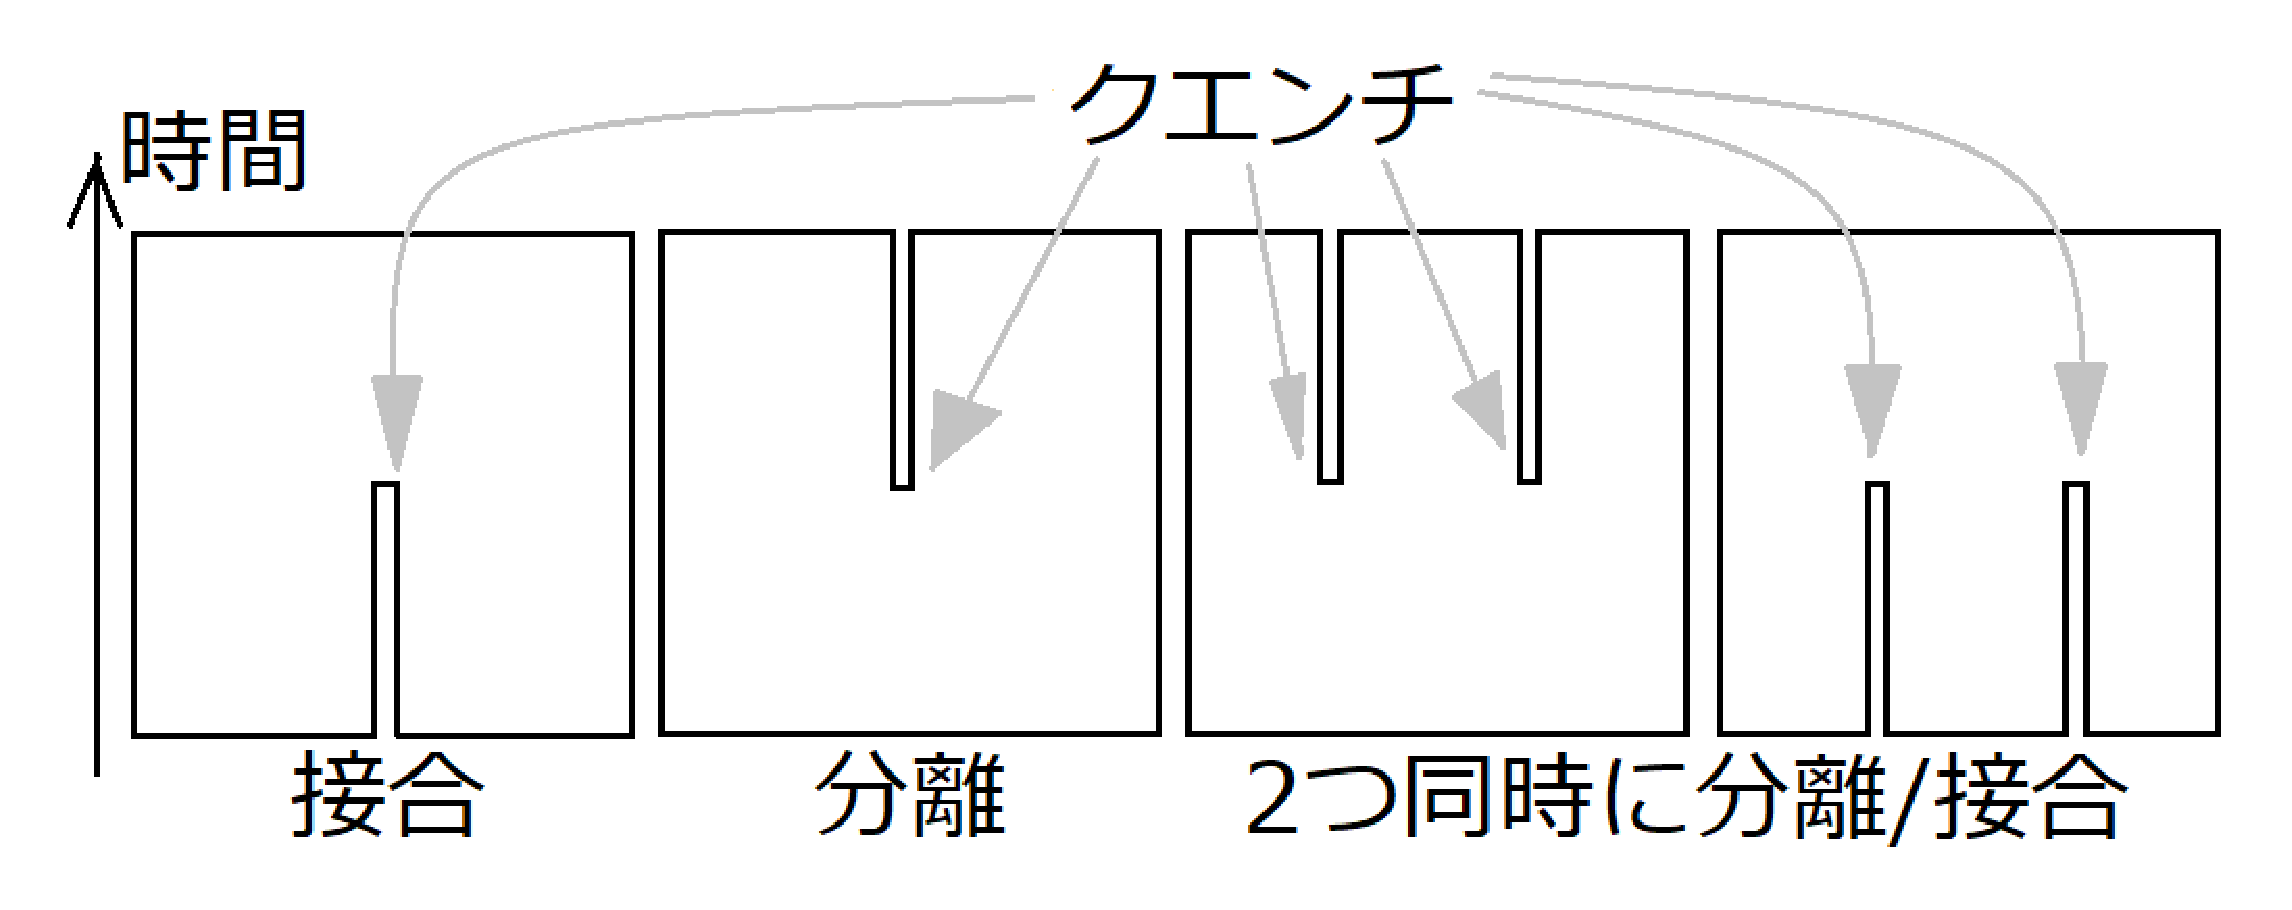
\includegraphics[width=0.7\linewidth]{quenchfig.pdf}
\end{figure}

以下に2つの論文で解析した内容の表をまとめる。
\begin{table}[H]
	\centering
	\begin{tabular}{|c||c|c|c|c|}\hline\hline
		  & 接合 & 分離 & 2重接合 & 2重分離 \\ \hline
		零質量自由Dirac場のEE & $\bigcirc$ & $\bigcirc$ & $\bigcirc$ & $\bigcirc$ \\
		重力双対を持つCFTのEE & $\bigcirc$ & $\bigcirc$ & $\bigcirc$ & $\bigcirc$ \\
		重力双対の測地線の描像 & $\bigcirc$ & $\bigcirc$ & $\bigcirc$ &  \\ \hline
	\end{tabular}
\end{table}

本論文では、分離クエンチと2重分離クエンチに焦点をあてて、その解析結果を解説する。分離クエンチは\cite{gring2012relaxation}で、二重井戸型ポテンシャルを用いて1次元冷却原子気体を2つに分離することで実験されており、実験への応用を考える上でも興味深い。また、格子系を分離クエンチしたときのEEの計算は\cite{Zamora_2014}で研究されていた。我々の解析はその連続理論版にあたる。

重力双対を持つCFTのEEの計算は、笠-高柳公式を用いて測地線の長さを計算することで行った。このとき、多くの場合で測地線はPoincare領域で覆われる領域を出て、AdS空間の大域的なトポロジーに関係することがわかった。この現象はHartman,Maldacena\cite{hartman2013time}などによって別の問題設定でも起きることが知られている。

零質量自由Dirac場はカオス性のない``可積分"な理論であるのに対して、重力双対を持つCFTは非常に強いカオス性を持つことが知られている\cite{Maldacena:2015waa}。これらのEEの振る舞いを比較することで、重力双対を持つCFTは、カオス的でない零質量自由Dirac場に比べて急速に熱平衡化が起きることが分かった。

また、2重分離クエンチでのエンタングルメントエントロピーの解析により、3次元重力理論の境界におけるboundary gravitonの自由度の存在を確認し、引力相互作用が働いていることを予想した。

\section*{本論文の構成}
本論文の構成は以下のとおりである。\ref{chap:adscftreview}章では2次元共形場理論やその具体例である自由場の理論と、3次元漸近的AdS空間の理論をして、それらのAdS$_3$/CFT$_2$対応を解説する。また本研究で用いたAdS/BCFTの処方についても解説する。\ref{chap:EEreview}章では場の理論におけるエンタングルメントの定義を述べた後、2次元共形場理論のエンタングルメントエントロピーと、AdS$_3$/CFT$_2$対応についての笠-高柳公式を解説する。

\ref{chap:singlquench}章では我々の研究\cite{Shimaji:2018czt}に基づいて、直線上の2次元共形場理論の真空を分離クエンチしたときのエンタングルメントエントロピーの時間発展を解析し、その重力双対の描像を調べる。このとき分離によって、双対なAdS$_3$空間に非常に重い障害が出来ることを見る。

\ref{chap:doublequench}章では我々の研究\cite{Caputa:2019avh}に基づいて、直線上の2次元共形場理論の真空を2重分離クエンチしたときのエンタングルメントエントロピーの時間発展を解析する。\ref{chap:singlquench}の解析から、共形場理論の2つの分離に対応してその双対なAdS$_3$空間には2つの重い障害が生じると考えられ、それらはAdS$_3$の境界に生じる重力相互作用で引き合うと考えられるが、このことをエンタングルメントエントロピーの振る舞いから解釈する。
